\PassOptionsToPackage{unicode}{hyperref}
\PassOptionsToPackage{naturalnames}{hyperref}
\documentclass[aspectratio=169]{beamer} 

%%% FONT SELECTION %%%%%%%%%%%%%%%%%
\usepackage[T1]{fontenc}
\usepackage{lmodern}

%%%%%%%%%%%%%%%%%%%%%%%%%%%%%%%%%%%%

\usepackage{color}
\usepackage{url}
\usepackage{amsmath}
\usepackage{amssymb}
\usepackage{booktabs}
\usepackage{siunitx}

\usepackage{epstopdf}
\usepackage{graphicx}
\graphicspath{{./images/}}

% load layout
\usepackage{TeiPel_En_Beamer_Layout}
\setTeipelLayout{newlogo}

%%%%%%%%%%%%%%%%%%%%%%%%%%%%%%%%%%%%%%%%%%%%%%%%%%%%%%%%%%%%
% Thesis Info
%%%%%%%%%%%%%%%%%%%%%%%%%%%%%%%%%%%%%%%%%%%%%%%%%%%%%%%%%%%%
	\title[Analisi spettrale di eventi SEP e stime della dose per missioni interplanetarie]{Analisi spettrale di eventi SEP\\e stime della dose per missioni interplanetarie}	
	\author[S. Dolci]{Stefano Dolci}
	\supervisor{Relatore}{Prof.~Massimo Gervasi}{Correlatore: Dott.~Stefano Della Torre}
	\presentationDate{26 marzo 2026}
\setbeamersize{text margin left=0.5em, text margin right=0.5em}

\begin{document}

% --- Title page (senza footer) ---
{
\setbeamertemplate{footline}{}
\begin{frame}[plain]
  \titlepage
\end{frame}
}

% --- Indice con immagine a fianco ---
\begin{frame}{Indice}
    \begin{columns}
        \begin{column}{0.55\textwidth}
            \linespread{1.5}\selectfont
            \tableofcontents
        \end{column}
        \begin{column}{0.4\textwidth}
            \centering
            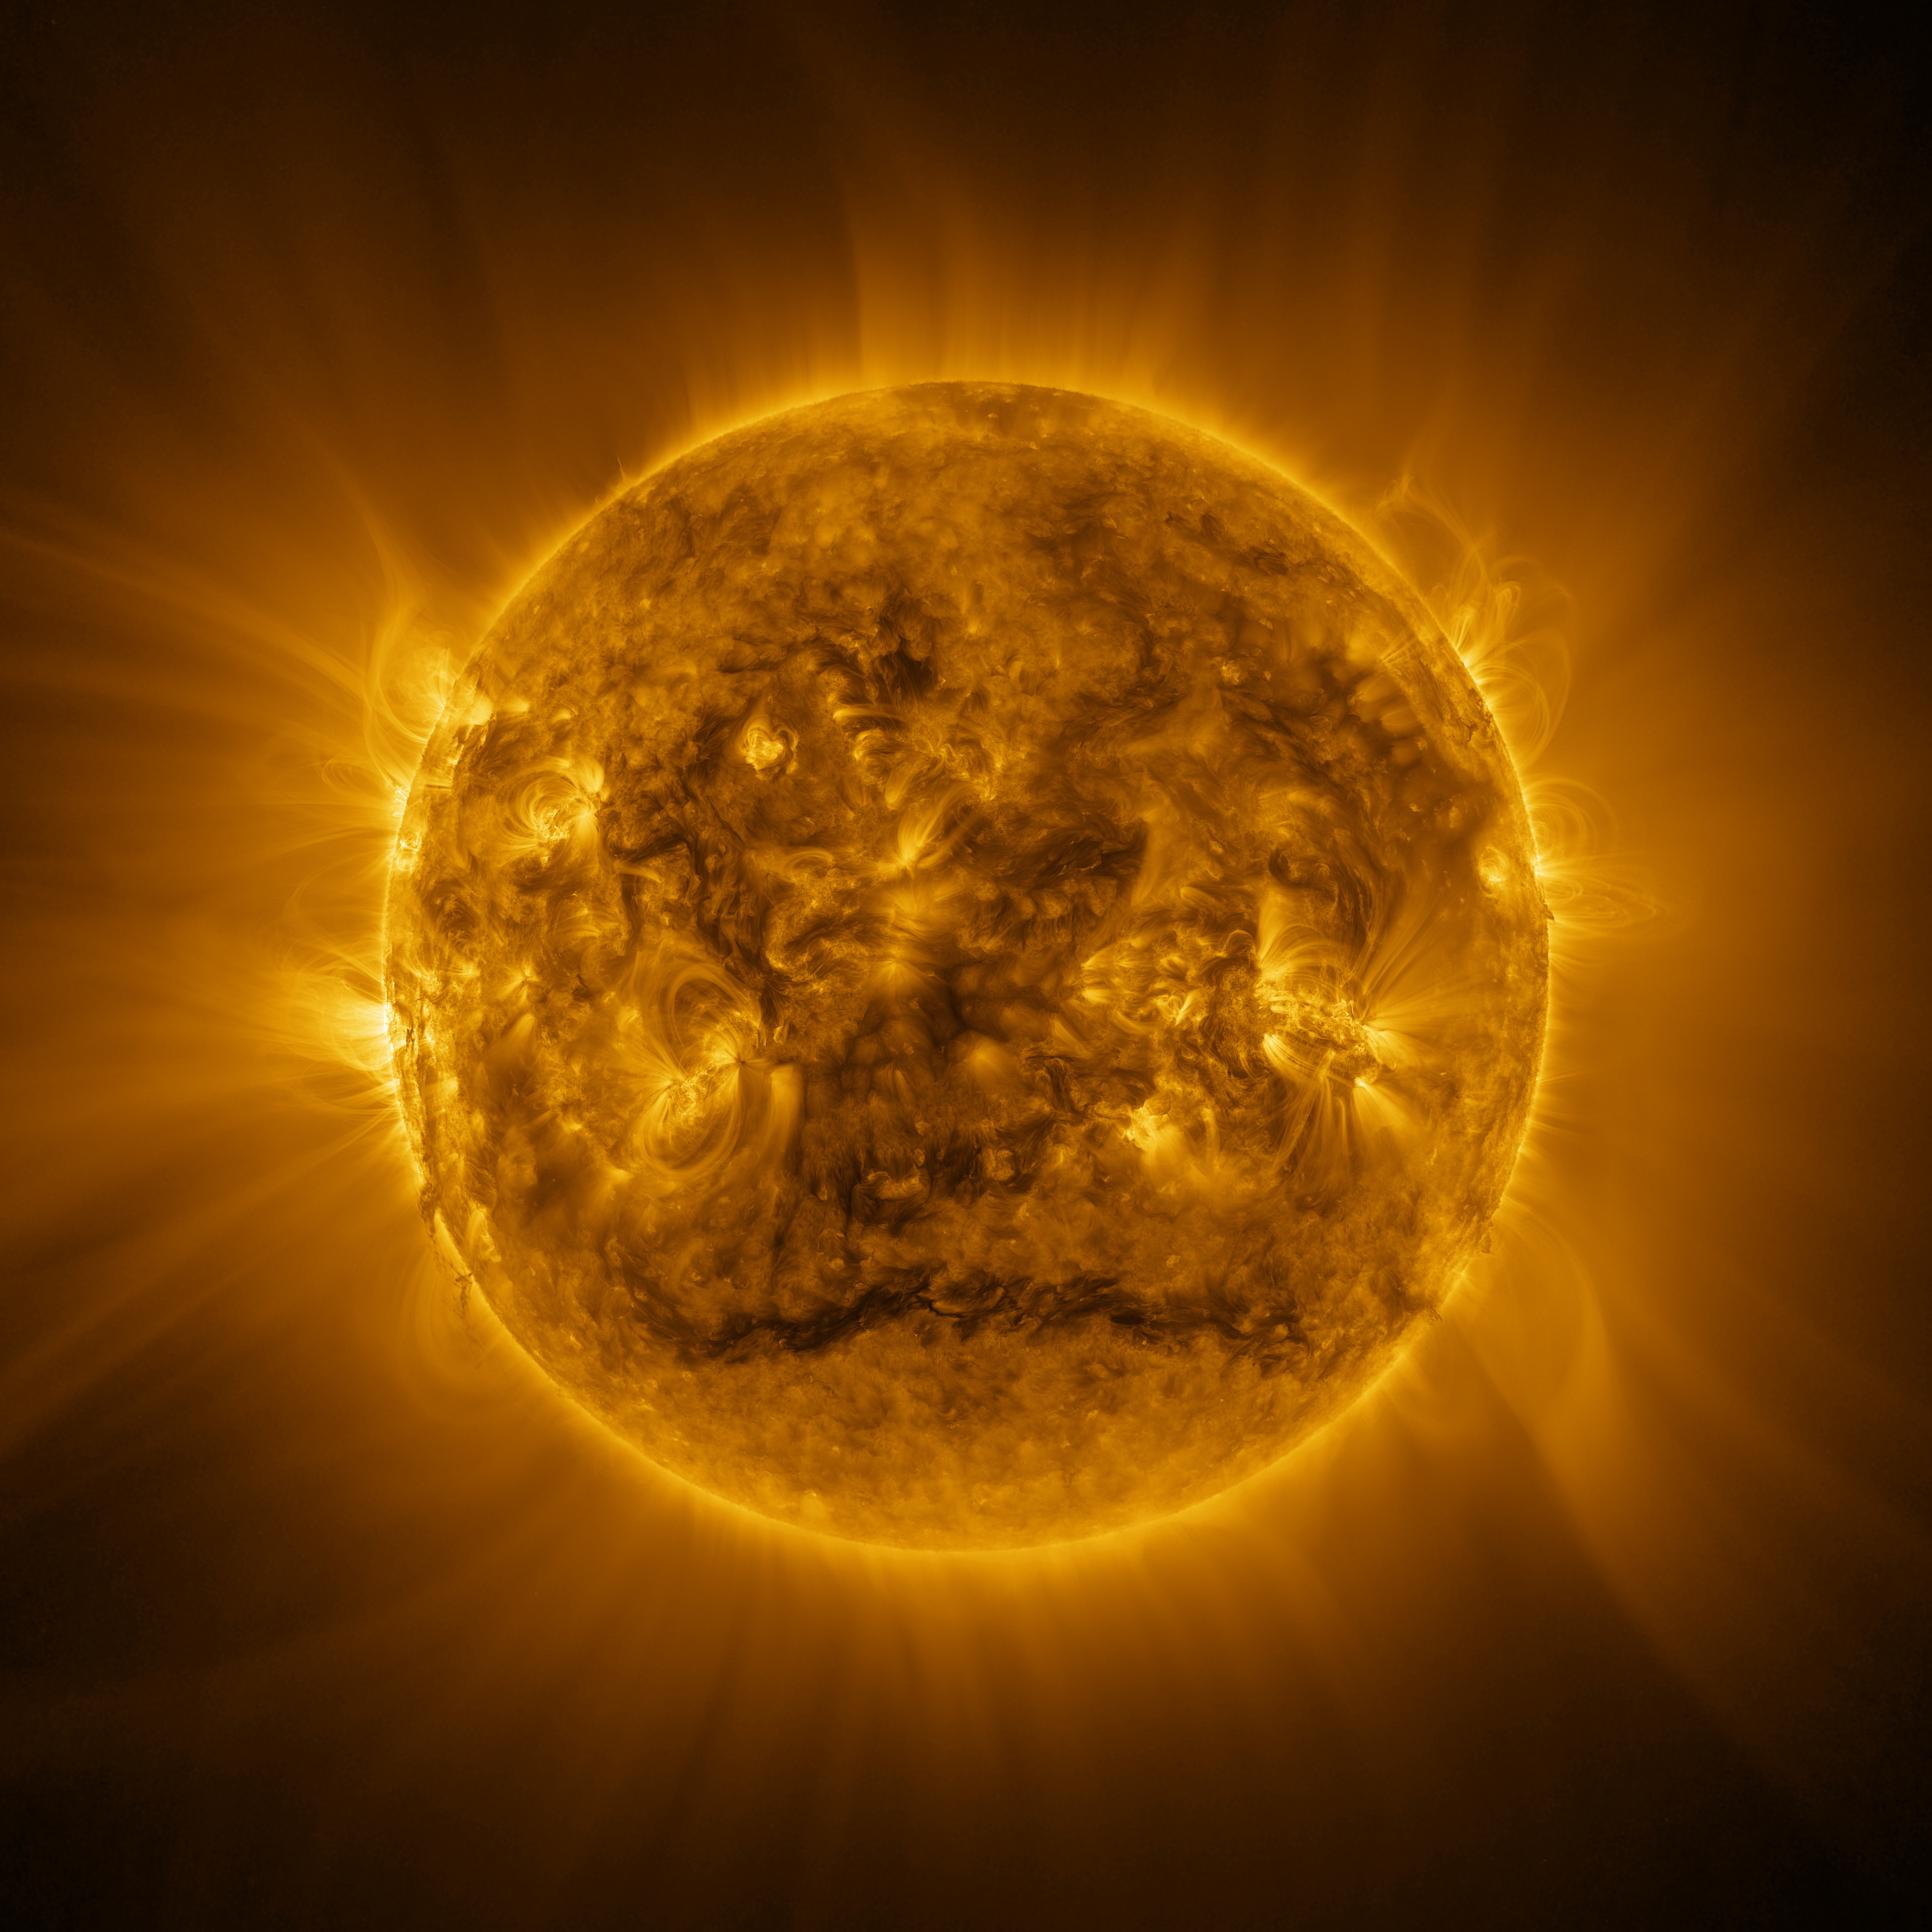
\includegraphics[width=\textwidth,keepaspectratio]{Solar_Orbiter_s_widest_high-res_view_of_the_Sun.jpg}
        \end{column}
    \end{columns}
\end{frame}

%%%%%%%%%%%%%%%%%%%%%%%%%%%%%%%%%%%%%%%%%%%%%%%%%%%%%%%%%%%%%%%%
\section{Introduzione}
%%%%%%%%%%%%%%%%%%%%%%%%%%%%%%%%%%%%%%%%%%%%%%%%%%%%%%%%%%%%%%%%

\begin{frame}{Contesto}
    \begin{columns}
        \begin{column}{0.58\textwidth}
            \begin{itemize}
                \item Radiazione ionizzante:
                \begin{itemize}
                    \item \textbf{GCR}: Galactic Cosmic Rays
                    \item \textbf{SEP}: Solar Energetic Particles
                \end{itemize}
                \item Protoni ed elettroni (energie keV-GeV)
                \item Natura stocastica $\Rightarrow$ approccio probabilistico
            \end{itemize}
            \vspace{0.5em}
            \begin{block}{Obiettivo}
                Stimare la dose da protoni SEP che una sonda accumulerebbe per un transito Terra--Marte.
            \end{block}
        \end{column}
        \begin{column}{0.38\textwidth}
            \centering
            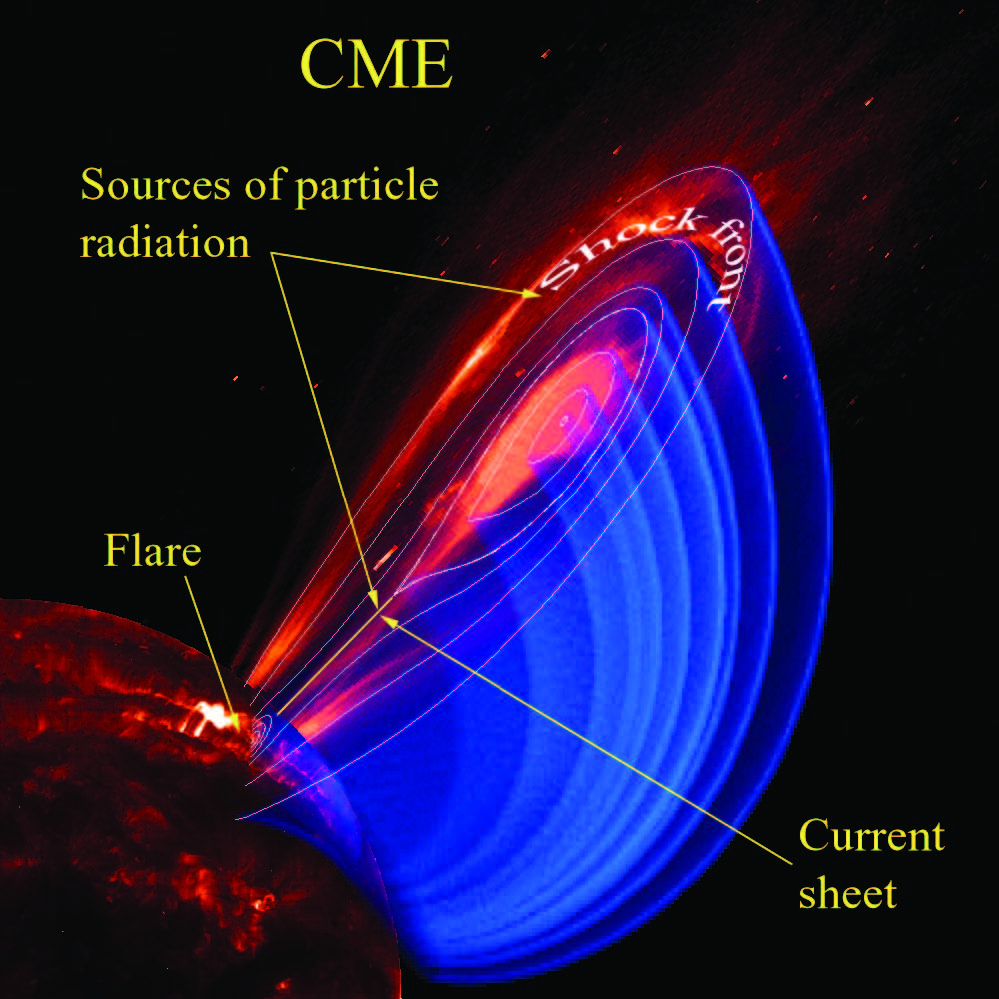
\includegraphics[width=\textwidth,keepaspectratio]{sep_fig2 (1).jpg}
            {\tiny Fonte: ESA/SEPEM \cite{sepem_intro}}
        \end{column}
    \end{columns}
\end{frame}
\begin{frame}{Come si simula la dose da SEP?}
    \begin{columns}[T]
        \begin{column}{0.30\textwidth}
            \uncover<1->{%
            \begin{block}{\centering 1. Dati}
                \centering
                {\small GOES, ACE, STEREO\\Flussi differenziali}
            \end{block}}
        \end{column}
        \begin{column}{0.30\textwidth}
            \uncover<2->{%
            \begin{block}{\centering 2. Flussi}
                \centering
                {\small Preprocessing:\\background, ricampionamento}
            \end{block}}
        \end{column}
        \begin{column}{0.30\textwidth}
            \uncover<3->{%
            \begin{block}{\centering 3. Fit spettrale}
                \centering
                {\small Band / Ellison-Ramaty\\$\chi^2$ + Monte Carlo}
            \end{block}}
        \end{column}
    \end{columns}

    \vspace{0.5em}

    \begin{columns}[T]
        \begin{column}{0.30\textwidth}
            \uncover<4->{%
            \begin{block}{\centering 4. SR-NIEL}
                \centering
                {\small Trasporto in Al\\Dose in Si (TID)}
            \end{block}}
        \end{column}
        \begin{column}{0.30\textwidth}
            \uncover<5->{%
            \begin{block}{\centering 5. $D(J)$}
                \centering
                {\small $D = 10^a \cdot J(>E_0)^b$\\Funzione di trasferimento}
            \end{block}}
        \end{column}
        \begin{column}{0.30\textwidth}
            \uncover<6->{%
            \begin{block}{\centering 6. SAPPHIRE}
                \centering
                {\small Modello probabilistico\\100\,000 timeline virtuali}
            \end{block}}
        \end{column}
    \end{columns}
\end{frame}


\begin{frame}{Come si simula la dose da SEP?}
	\begin{itemize}
		\item Effetti \textbf{cumulativi}: TID e Displacement Damage Dose (DDD)
		\begin{itemize}
			\item Accumulo di carica nell'ossido di gate $\Rightarrow$ deriva dei parametri elettrici
		\end{itemize}
		\item Effetti \textbf{singoli}: Single Event Effects (SEE)
		\item Schermatura standard: alluminio, tipicamente 5--10~g/cm$^2$
		\item Dose misurata in Gray: $\text{TID} = E_{\text{dep}}/m$ \quad [1~Gy = 1~J/kg]
	\end{itemize}
	% >>> INSERIRE: figura transistor MOS pre/post irradiazione (Fig. 1.2)
\end{frame}

%%%%%%%%%%%%%%%%%%%%%%%%%%%%%%%%%%%%%%%%%%%%%%%%%%%%%%%%%%%%%%%%
\section{Analisi spettrale}
%%%%%%%%%%%%%%%%%%%%%%%%%%%%%%%%%%%%%%%%%%%%%%%%%%%%%%%%%%%%%%%%

\begin{frame}{Dataset: 8 eventi SEP (1972--2024)}
	\begin{itemize}
		\item Selezionati i due eventi pi\`u intensi per ciclo solare (cicli 20--25)
		\item Dati da: GOES (EPS/HEPAD), ACE (EPAM), IMP-8, STEREO-A (LET/HET)
		\item Preprocessing: ricampionamento 30~min, sottrazione background ($\mu + 3\sigma$)
	\end{itemize}
	\vspace{0.5em}
	% >>> INSERIRE: tabella 8 eventi (date, rivelatori, note)
\end{frame}

\begin{frame}{Modelli spettrali}
	% >>> INSERIRE: formule Band function e Ellison-Ramaty
	\begin{itemize}
		\item \textbf{Band function}: doppia legge di potenza --- 4 parametri ($A$, $\gamma_a$, $\gamma_b$, $E_0$)
		\item \textbf{Ellison-Ramaty}: legge di potenza con cutoff esponenziale --- 3 parametri ($K$, $\gamma$, $E_R$)
		\item Fit in \textbf{spazio logaritmico} con $\chi^2$ ridotto (Levenberg--Marquardt)
		\item Propagazione errori: \textbf{Monte Carlo parametrico} ($N_{\text{MC}} = 1000$) dalla matrice di covarianza
	\end{itemize}
\end{frame}

\begin{frame}{Esempio fit: Ottobre 2003 (Halloween Storm)}
	% >>> INSERIRE: plot spettro Oct 2003 (Fig. 2.7)
	\begin{itemize}
		\item Flare X17 + X10, CME $>$~2000~km/s
		\item Dati: ACE/EPAM + GOES-11 (EPS+HEPAD)
		\item $\chi^2_\nu = 2.20$, \; $\gamma_a = 1.01\pm0.06$, \; $\gamma_b = 3.71\pm0.11$
		\item $E_{\text{break}} = 43$~MeV --- spettro duro, dose significativa dietro schermature spesse
	\end{itemize}
\end{frame}

\begin{frame}{Risultati: fluenze integrali}
	% >>> INSERIRE: Tabella 2.2 (fluenze integrali omnidirezionali)
	\begin{itemize}
		\item Quasi 3 ordini di grandezza in $J(> 10~\text{MeV})$: da $5.3\times10^{10}$ a $7.1\times10^{7}$~cm$^{-2}$
		\item $\gamma_a \sim 0.9$--$1.3$: firma dell'accelerazione da shock/CME
		\item Nessuna correlazione semplice tra fluenza totale e durezza spettrale
	\end{itemize}
\end{frame}

%%%%%%%%%%%%%%%%%%%%%%%%%%%%%%%%%%%%%%%%%%%%%%%%%%%%%%%%%%%%%%%%
\section{Calcolo della dose}
%%%%%%%%%%%%%%%%%%%%%%%%%%%%%%%%%%%%%%%%%%%%%%%%%%%%%%%%%%%%%%%%

\begin{frame}{Calcolo TID con SR-NIEL}
	\begin{itemize}
		\item Piattaforma SR-NIEL: propagazione CSDA dello spettro attraverso schermatura
		\item Configurazione: protoni su Al (10~g/cm$^2$), dose in Si
		\item Due geometrie:
		\begin{itemize}
			\item Planare ($\pi$~sr) --- flusso unidirezionale su superficie piana
			\item Sferica ($4\pi$~sr) --- flusso isotropo su guscio sferico
		\end{itemize}
		\item Incertezze: bande MC (16\%--84\%) $\oplus$ 5\% stopping power SRIM
	\end{itemize}
	% >>> INSERIRE: schema geometria planare/sferica (Fig. 3.1 / 3.2)
\end{frame}

\begin{frame}{Funzione di trasferimento $D(J)$}
	% >>> INSERIRE: formula D = 10^a * J^b e plot D vs J (Fig. 3.6)
	\begin{itemize}
		\item Relazione empirica: $D(J) = 10^a \cdot J(> E_0)^b$
		\item Soglia ottimale: $J(>100)$~MeV (sferica), $J(>60)$~MeV (planare)
		\item Da $J(>30)$ a soglia ottimale: scatter da $\pm35\%$ a $\pm10\%$
		\item Validazione LOO-CV: RMSE $\pm 9.8\%$ (planare), $\pm 13.6\%$ (sferica)
	\end{itemize}
\end{frame}

%%%%%%%%%%%%%%%%%%%%%%%%%%%%%%%%%%%%%%%%%%%%%%%%%%%%%%%%%%%%%%%%
\section{Risultati}
%%%%%%%%%%%%%%%%%%%%%%%%%%%%%%%%%%%%%%%%%%%%%%%%%%%%%%%%%%%%%%%%

\begin{frame}{Stime TID con SAPPHIRE}
	% >>> INSERIRE: Tabella 4.1 (versione ridotta) e/o Fig. 4.1
	\begin{itemize}
		\item SAPPHIRE (ESA/SEPEM): modello probabilistico, 100\,000 timeline virtuali
		\item Scenario di riferimento (sferica, 0.7~yr, max solare, 90\% CL):
		\begin{itemize}
			\item $D_{\text{sfer}} = 62.1 \pm 6.2$~mGy
		\end{itemize}
		\item Range completo: da 2.3~mGy (min solare) a 137~mGy (1~yr, 95\% CL)
		\item Fattore dominante: \textbf{fase del ciclo solare} ($\sim$2 ordini di grandezza)
	\end{itemize}
\end{frame}

\begin{frame}{Confronto SEP/GCR e validazione MSL/RAD}
	% >>> INSERIRE: Tabella 5.1 (SEP vs GCR)
	\begin{itemize}
		\item MSL/RAD (transito 253~gg, ciclo 24 debole): 24.7~mGy da 5 eventi SEP
		\item Rapporto SEP/GCR (0.7~yr, 90\% CL):
		\begin{itemize}
			\item Massimo solare: $\sim 1.6$ --- \textbf{SEP dominano}
			\item Minimo solare: $\sim 0.07$ --- GCR dominano
		\end{itemize}
		\item Risultati compatibili con misure in-situ
	\end{itemize}
\end{frame}

\begin{frame}{Scaling radiale: orbita di Hohmann}
	% >>> INSERIRE: plot traiettoria r(t) (Fig. 5.2) e/o Tabella 5.3
	\begin{itemize}
		\item Orbita di trasferimento: $r$ varia da 1.0 a 1.52~AU in 259~giorni
		\item Due approcci:
		\begin{itemize}
			\item Scaling geometrico ($J \propto r^{-\alpha}$): riduzione 30--50\%
			\item SOLPENCO2 (trasporto MHD): riduzione $\sim 20\%$
		\end{itemize}
		\item Con SOLPENCO2: $D_{\text{plan}} \approx 30$~mGy --- compatibile con MSL/RAD ($\sim$24.7~mGy)
	\end{itemize}
\end{frame}

%%%%%%%%%%%%%%%%%%%%%%%%%%%%%%%%%%%%%%%%%%%%%%%%%%%%%%%%%%%%%%%%
\section{Conclusioni}
%%%%%%%%%%%%%%%%%%%%%%%%%%%%%%%%%%%%%%%%%%%%%%%%%%%%%%%%%%%%%%%%

\begin{frame}{Conclusioni}
	\begin{enumerate}
		\item Analisi spettrale di \textbf{8 eventi SEP} (1972--2024) con Band e Ellison-Ramaty
		\item Funzione $D(J)$ ottimizzata: TID stimabile con $\sim$10\% dalla sola fluenza integrale
		\item TID per transito Terra--Marte (0.7~yr, max solare, 90\% CL):
		\begin{itemize}
			\item 62.1$\pm$6.2~mGy (sferica), \; 37.3$\pm$2.9~mGy (planare) a 1~AU
			\item Con SOLPENCO2: $\sim$46--30~mGy
		\end{itemize}
		\item SEP dominano durante massimo solare (SEP/GCR $\sim 1.6$)
		\item Soglia energetica ottimale: risultato chiave per mission planning
	\end{enumerate}
	\vspace{1em}
	\centering
	\Large Grazie per l'attenzione!
\end{frame}

%%%%%%%%%%%%%%%%%%%%%%%%%%%%%%%%%%%%%%%%%%%%%%%%%%%%%%%%%%%%%%%%
% BACKUP SLIDES (non contano nella numerazione)
%%%%%%%%%%%%%%%%%%%%%%%%%%%%%%%%%%%%%%%%%%%%%%%%%%%%%%%%%%%%%%%%
\appendix

\begin{frame}{Backup: dosi per tutti gli eventi}
	% >>> INSERIRE: Tabella 3.1 completa (fluenze + TID planare/sferica)
\end{frame}

\begin{frame}{Backup: parametri fit completi}
	% >>> INSERIRE: tabella riassuntiva parametri spettrali 8 eventi
\end{frame}

\begin{frame}{Backup: validazione LOO-CV}
	% >>> INSERIRE: Fig. 3.7 (prediction error per le 4 configurazioni)
\end{frame}


\begin{frame}[allowframebreaks]{Riferimenti}
    \bibliographystyle{plain}
    \bibliography{bibliography}
\end{frame}

\end{document}
